
	\chapter{序論}
    \section{研究の背景と目的}
    近年,AI分野は急速な発展を続けている.スマートスピーカなどの対話型のAIがGoogleやAmazon,IBMによって商品化され,現在ではスマートフォンにもSiriというAIが搭載されるなどその存在は非常に身近になっており,その種類も非常に多岐にわたる.
    \begin{figure}[h]
        \begin{screen}
        \begin{center}
            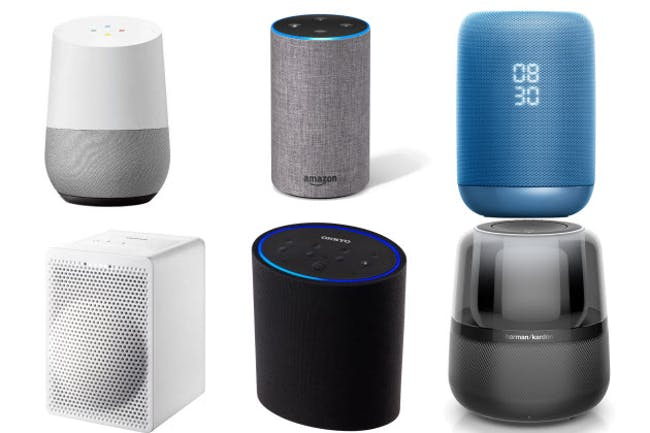
\includegraphics[scale=0.5, clip]{./img/smartspeaker_list.jpg}
            \caption{magentaによるMIDI音楽データ生成までのプロセス}
            \label{fig:magentaによるMIDI音楽データ生成までのプロセス}
        \end{center}
        \end{screen}
    \end{figure}\\
    また囲碁や将棋,チェスなどの競技においても,プロに勝利するなどその精度は以前から高いが,そのAIは一つの競技でしか使用できない特化型人工知能(AGI)であった.
    しかし,英DeepMindが発表したAlphaZeroという様々なボードゲームに対応できる汎用性を持ったAIが発表され,汎用人工知能(GAI)の成長も著しい.芸術の分野ではまだ発展途上ではあるが,絵画や音楽に関してもAIを用いて新しい作品を作るものが出回っている.\\
     このようにAIの発展は様々な分野においてその成果を上げており,今後は業務の効率化や補助だけにとどまらず,自動車の自動運転や医療の現場でも人間の手よりも高精度なものとして活躍することが期待されている.\\
    本研究ではAIによる楽曲生成についての実証実験を行う.Googole brainによって公開されているMagentaを用いて学習データやノード数による楽曲の生成結果の違いを比較,検証し,AIによる楽曲制作が有用なものか調査する.\\
    \section{本論文の構成}
    本論文の構成は以下の通りである.\\
    第1章では本論文の背景と目的について述べている.\\
    第2章では本論文で利用する理論について述べている.\\
    第3章では実験内容について述べている.\\
    第4章では楽曲制作について述べている.\\
    第5章ではAIを用いた楽曲制作についての本研究の結論について述べている.\\    